\section{Modellazione}
Un modello \`e un astrazione del nostro sistema, modelliamo il nostro \sw\ perch\`e con
il tempo, la dimensione dei sistemi \sw\ \`e cresciuta di molto.

Per questo motivo grazie a queste semplificazioni, riusciamo a modellare sia Il
\textbf{dominio applicativo} e anche il \textbf{dominio della soluzione}

\subsection{UML}
UML(Uniform Modelling Language) \`e un linguaggio di modellazione utilizzato in tutte le fasi
di sviluppo (analisi, progettazione, etc\dots). 
Nasce alla fine degli anni 80 dal OMG (Object Management Group).
I modelli UML si dividono in :
\begin{itemize}
    \item Modelli Strutturali o Statici:
        Modellano gli aspetti statici del sistema, quindi le parti che lo compongono e le interazioni 
    \item Modelli Comportamentali o Dinamici:
        Descrivono i comportamenti del nostro sistema, ad esempio scenari di utilizzo
    \item Modelli di interazione:
        Descrivono le vari interazioni in uno scenario (Sequence Diagram)
\end{itemize}
\begin{figure}[htbp]
    \centering
    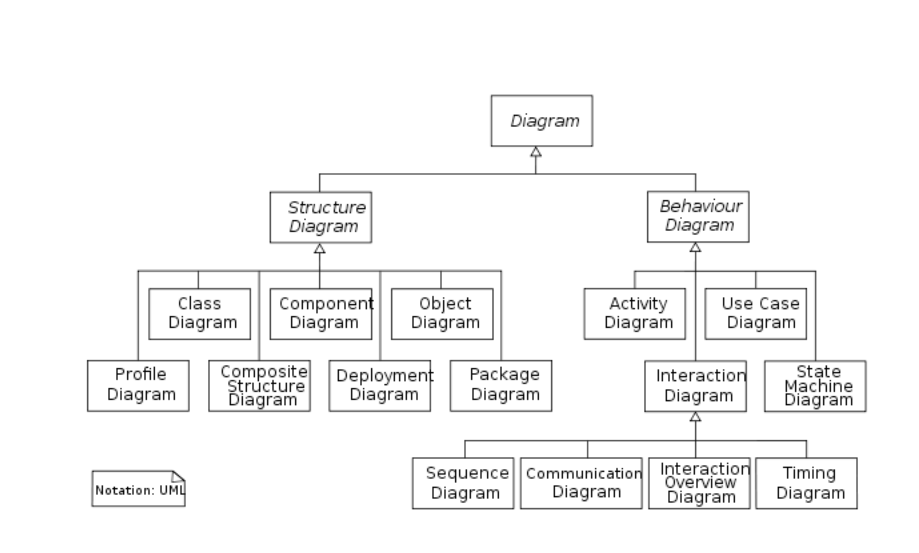
\includegraphics[scale=0.6]{Modelli_uml.PNG}
    \caption{Diagrammi Uml}
    \label{fig:uml}
\end{figure}
\subsection{Modelli Strutturali}
Introduciamo adesso i modelli \emph{strutturali}, che ripetendo, modellano gli aspetti strutturali
del nostro sistema ne fanno parte:
\begin{itemize}
    \item Class Diagram o diagramma delle classi
    \item Component Diagram
    \item Object Diagram
    \item Package Diagram
    \item Deployment Diagram
\end{itemize}
\subsubsection{Class Diagram}
Il diagramma delle classi modella la realta' del nostro sistema.

Il modello segue ampiamente la Object Oriented Programming (OOP).Infatti utilizza ampiamente
il concetto di classe, oggetto, eridetariet\`a e polimorfismo.
Il class Diagram viene Utilizzato sia in fase di analisi che di progettazione.
infatti distinguiamo in:
\begin{itemize}
    \item System Domain Model (SDM):
        Modello concettuale, serve a modellare le classi del nostro sistema, quindi le entita
        che partecipano alla soluzione
    \item System Model:
        Modello pi\`u dettagliato, contiene tutte le classi che partecipano alla soluzione, 
        anche quelle di supporto, ad esempio librerie di matematica, librerie per UI, etc\dots
\end{itemize}
\subsubsection{Object Diagram}
L'object diagram e' molto simile al class diagram, almeno nella notazione.

ma invece di modellare la classi e quindi la realta'.
Modella una \textbf{fotografia} in un istante, del class diagram, quindi modelliamo gli
oggetti e le loro interazioni in un particolare scenario.

E' utilizzato per esplicitare in modo chiaro le interazioni tra le classi in uno scenario, 
quindi e' molto usato nel debugging.

\subsubsection{Package Diagram}
Il package non e' altro che un contenitore di classi,
si usano per racchiudere classi \textbf{logicamente}.

Attenzione e' un raggruppamento LOGICO NON FISICO(vedere component diagram).

I package tra di loro condividono lo stesso \textbf{Spazio dei nomi}.

\subsubsection{Component diagram}
Il component diagram e' molto simile al package diagram, ma invece di raccogliere le classi
logicamnete, le va a raccogliere fisicamente, quindi modella l'effettiva file structure del progetto
.

Particolare importanza e' data al concetto di interfaccia, infatti i COMPONENTI dialogono ctramite interfaccia.

\subsubsection{Deployment Diagram}
Il deployment diagram mostrano l'architettura fisica del sistema.
Gli elementi che modelliamo sono chaiamati NODI(Pc, Server etc\dots). E sono collegati con archi
che rappresentano il canale di comunicazione tra di loro.

\subsection{Diagrammi comportamentali}
I diagrammi comportamentali, o dinamici, abbiamo detto modellano gli aspetti dinamici, quindi ad esempio
scenari di un caso d'uso.

\begin{itemize}
    \item Use Case Diagram
    \item Activity Diagram
    \item State Chart Diagram
    \item Sequence Diagram
    \item Communication Diagram
    \item Interaction Overview Diagram
\end{itemize}
\subsubsection{Use Case Diagram}
Un caso d'uso non e' altro che un interazione hw/sw con un attore per raggiungere un risultato.

Un attore non e' altro che una persona, un altro sistema che interagisce col sistema.

Dividiamo in:
\begin{itemize}
    \item Attore primario: attore che fornisce uno stimolo per avviare il caso d'uso 
    \item Attore secondario: attore che interagisce col sistema dopo l'avvio, quindi una figura secondaria
        ma comunque necessaaria per la terminazione del caso d'uso
\end{itemize}
Il caso d'uso pero non esplicita la sequenza di azioni per irsolvere il problema  ma solo cosa.

Quindi e' molto generico e vago, e poi con la definizione degli SCENARIO, possiamo definire proprio
la sequenza di azioni.

Di parrticolare importanza sono gli scenari alternativi, scenari che avvengono solo in particolari
condizioni spesso di errore ad esempio.

Uno degli scopi e' anche quello di definire un CONFINE PER IL MIO SISTEMA, cioe' quali sono le 
funzionalita' da produrre, responsabilita' del sistema, e cosa e' esterno al sistema.

\subsubsection{Sequence diagram}
Il sequence diagram e' un modello dinamico, che esplicita le sequenze di azioni da svolgere
per terminare un caso d'uso.
Quindi partiamo da uno o piu' attori e poi le vari interazioni tra gli oggetti del sistema.

Il sequence puo' essere usato sia in fase di analisi che di progettazione(sequence di dettaglio).
Importante nel sequence e' l'esplicitazione del tempo!!.

\subsubsection{Communication diagram}
Molto simile al sequence, infatti utilizza le stesse notazioni, ma invece di esplicitare le azioni in verticale.
Il tempo viene rappresentato da una NUMERAZIONE dei messaggi.
\subsubsection{State Chart Diagram}
